% Results chapter: presents empirical findings without interpretation.

\section{Schema Change Detection Results (RQ1)}
\label{sec:results-detection}

This section reports quantitative results for the schema change detection component in the controlled NYC taxi evolution scenarios. The focus is on precision, recall, and F\(_1\)~score for added, removed, and renamed columns when comparing detector outputs against ground-truth change sets.

\subsection{NYC Taxi V1~\texorpdfstring{$\rightarrow$}{->}~V2}

For the V1~$\rightarrow$~V2 evolution at the source level, the detector is evaluated on the change set constructed for the \path{yellow_base_v1.csv} and \path{yellow_base_v2.csv} files. The ground truth comprises a rename of \path{trip_distance} to \path{trip_km}, the addition of \path{tip_ratio}, removal of \path{payment_type}, and a type change of \path{VendorID} from integer to string, as summarised in Table~\ref{tbl:taxi-v1-v2-changes} in Chapter~\ref{sec:method-data}.

The evaluation JSON file \path{results/schema_detection_eval.json} records that the detector recovers the designed rename and added column with perfect precision and recall, and correctly flags the overall change pattern, but does not report removed columns for this particular scenario. As a result, the F\(_1\)~scores for added and renamed changes are 1.0, while the score for removed columns is 0.0 because the ground-truth removal is not represented in the detector output for V1~$\rightarrow$~V2. This highlights both the strengths and limitations of the current heuristic-based removal detection for this schema pair.

\subsection{Canonical~\texorpdfstring{$\leftrightarrow$}{<->}~V2}

For the canonical~$\leftrightarrow$~V2 scenario, the detector is evaluated on the change set used for canonical ingestion experiments and stored in \path{results/canonical_changes_v2.json}. Here, the evolution is specified between the single-table canonical schema and the V2 source schema. The detector identifies two added canonical columns, eleven removed canonical columns, and one rename, all of which are captured in the ground-truth JSON.

Table~\ref{tbl:results-schema-metrics} summarises the quantitative metrics for this scenario. The detector achieves precision, recall, and F\(_1\)~scores of 1.0 for added, removed, renamed, and overall changes, indicating that it recovers the designed canonical--V2 evolution exactly for this flat tabular schema.

\begin{table}[h]
  \centering
  \caption{Schema change detection metrics for canonical~\texorpdfstring{$\leftrightarrow$}{<->}~V2 (from \texttt{results/canonical\_changes\_v2.json}).}
  \label{tbl:results-schema-metrics}
  \begin{tabular}{llll}
    \hline
    Change type & Precision & Recall & F\(_1\) \\
    \hline\hline
    Added columns   & 1.00 & 1.00 & 1.00 \\
    Removed columns & 1.00 & 1.00 & 1.00 \\
    Renamed columns & 1.00 & 1.00 & 1.00 \\
    Overall         & 1.00 & 1.00 & 1.00 \\
    \hline
  \end{tabular}
\end{table}

Figure~\ref{fig:schema-detection-canonical-v2} illustrates the outcome of the heuristic schema change detector for the canonical~$\leftrightarrow$~V2 scenario. The detector correctly classifies added columns (e.g.\ the two canonical-derived attributes), removed columns (the V2-only attributes that do not appear in the canonical schema), and the single rename (\texttt{trip\_km}~$\rightarrow$~\texttt{trip\_distance}), yielding the perfect precision, recall, and F\(_1\)~scores reported in Table~\ref{tbl:results-schema-metrics}.

\begin{figure}[htbp]
  \centering
  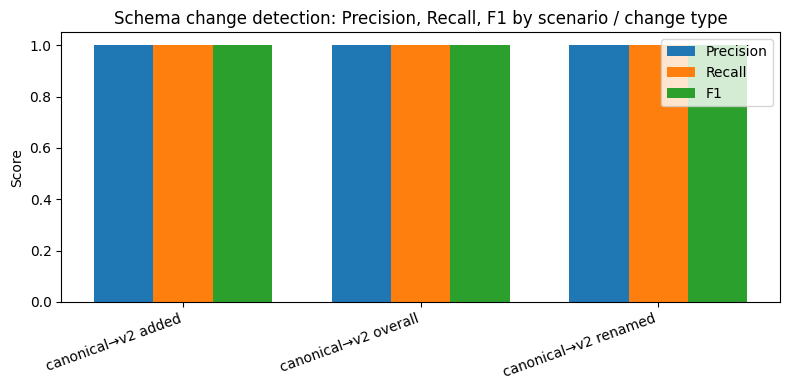
\includegraphics[width=0.85\textwidth]{figures/schema_detection_canonical_v2}
  \caption{Schema change detection result for the canonical~$\leftrightarrow$~V2 scenario. The heuristic detector identifies added canonical columns, removed V2-only columns, and the \texttt{trip\_km}~$\rightarrow$~\texttt{trip\_distance} rename, matching the ground-truth change set used for canonical ingestion.}
  \label{fig:schema-detection-canonical-v2}
\end{figure}

\subsection{Heuristic vs.\ RAG-LLM Detection for Canonical~\texorpdfstring{$\leftrightarrow$}{<->}~V2}

To assess whether schema change detection itself can be driven by a retrieval-augmented LLM rather than hand-crafted heuristics, a separate experiment compares the heuristic detector against the hosted \path{openai/gpt-oss-120b:groq} model on the same canonical~$\leftrightarrow$~V2 scenario. The LLM-based detector is prompted only with machine-readable schema descriptions for the V2 source schema and the canonical schema (column names, inferred dtypes, and sample values), and is asked to emit a JSON change set with the same structure as the heuristic output (added, removed, renamed, type changes). The resulting LLM predictions are then evaluated against the canonical change set in \path{results/canonical_changes_v2.json} using the same precision/recall/F\(_1\) metrics as above.

\begin{table}[h]
  \centering
  \caption{Schema detection F\(_1\) scores for heuristic vs.\ RAG-LLM detectors on the canonical~\texorpdfstring{$\leftrightarrow$}{<->}~V2 scenario. Both methods are evaluated against the canonical change set in \texttt{results/canonical\_changes\_v2.json}.}
  \label{tbl:results-schema-heuristic-vs-llm}
  \begin{tabular}{lll}
    \hline
    Method     & Change type      & F\(_1\) \\
    \hline\hline
    Heuristic  & Added columns    & 1.00 \\
    Heuristic  & Removed columns  & 1.00 \\
    Heuristic  & Renamed columns  & 1.00 \\
    Heuristic  & Overall          & 1.00 \\
    RAG-LLM (\path{gpt-oss-120B}) & Added columns   & 1.00 \\
    RAG-LLM (\path{gpt-oss-120B}) & Removed columns & 1.00 \\
    RAG-LLM (\path{gpt-oss-120B}) & Renamed columns & 1.00 \\
    RAG-LLM (\path{gpt-oss-120B}) & Overall         & 1.00 \\
    \hline
  \end{tabular}
\end{table}

For this controlled canonical~$\leftrightarrow$~V2 case, the RAG-LLM detector achieves the same perfect F\(_1\)~scores as the heuristic method for added, removed, and renamed columns. This indicates that, at least for relatively simple flat schemas where the evolution events are cleanly expressed in column-level metadata, a retrieval-augmented LLM can recover the designed change set as accurately as a specialised heuristic detector.


\section{Canonical Ingestion Results (RQ2)}
\label{sec:results-canonical}

This section reports results for canonical ingestion experiments in which deterministic and LLM-generated mappings ingest NYC taxi V2 data into the canonical target schema. The evaluation compares the LLM-generated canonical mappings against the deterministic baseline using row-count agreement, cell-level agreement (accuracy), null-mismatch counts, and per-column agreement.

\subsection{Deterministic Baseline}

The deterministic baseline mapping from any taxi schema version into the canonical schema is implemented in \path{etl/baseline_to_canonical.py}. For V2, the baseline ingests the down-sampled dataset of 93{,}679 rows into the \path{trips_canonical} table. By construction, baseline metrics for this mapping serve as the reference: 100\% cell-level agreement with itself, zero null mismatches, and 100\% per-column agreement across all canonical attributes, including derived columns such as \path{trip_duration_minutes} and \path{trip_revenue}.

In addition to defining the deterministic baseline algorithm, we empirically validate that it preserves the V2 data when ingesting into the canonical table. Concretely, we compare the baseline-normalised V2 CSV against the \path{trips_canonical} table for \texttt{source\_version = 'v2'} and \texttt{ingestion\_method = 'baseline'}. The row counts match exactly (93{,}679 rows in both), and summary statistics (means and sums) for schema-evolution columns such as \texttt{trip\_duration\_minutes}, \texttt{trip\_revenue}, \texttt{passenger\_count}, and \texttt{fare\_amount} are identical up to numerical precision.

\begin{figure}[htbp]
  \centering
  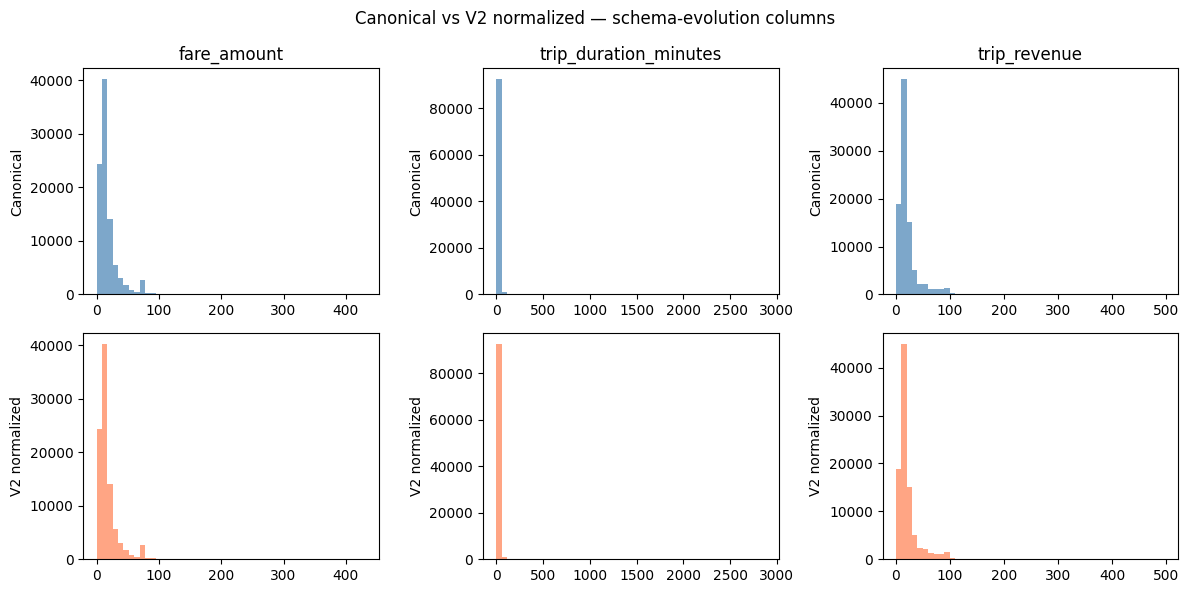
\includegraphics[width=0.9\textwidth]{figures/canonical_vs_v2_distributions}
  \caption{Distributions of key schema-evolution columns in the canonical table (\texttt{trips\_canonical}, V2 baseline) versus the baseline-normalised V2 CSV. For each column, the histograms for the canonical table (top row) and the normalised V2 data (bottom row) are visually indistinguishable, supporting that deterministic canonical ingestion preserves the original V2 data.}
  \label{fig:canonical-vs-v2-distributions}
\end{figure}

\subsection{LLM-Generated Canonical Mapping: \texttt{llama3}}
\label{sec:results-canonical-llama3}

The primary LLM evaluated for canonical ingestion is \path{llama3}, configured via the OpenAI-compatible interface in \path{ai/regenerate_mapping.py}. The evaluation JSON file \path{results/canonical_eval\_llama3.json} aggregates results across runs in which the LLM regenerates a canonical ingestion function for V2 from schema and change artefacts plus a reference transform snippet.

For the V2 scenario, the evaluation JSON file \path{results/canonical_eval\_llama3.json} records that the generated canonical ingestion mapping achieves:
%
\begin{itemize}
  \item a baseline row count of 93{,}679 and an LLM row count of 100{,}000, so \path{row_count_match = false},
  \item 93{,}679 rows compared cell-wise between baseline and LLM outputs,
  \item a cell agreement of 19.5\% across all compared cells,
  \item a null-mismatch count of 11{,}805, and
  \item heterogeneous per-column agreement, with some attributes (such as \path{tolls_amount}) showing high agreement while others (including temporal and derived columns) diverge substantially from the baseline.
\end{itemize}

These aggregate metrics align with Table~\ref{tbl:thesis-eval-summary} and illustrate that, without additional safeguards, \texttt{llama3} only partially reproduces the deterministic canonical mapping in the non-ablation runs.

\subsection{LLM-Generated Canonical Mapping: \texttt{mistral}}
\label{sec:results-canonical-mistral}

The \path{mistral} model is evaluated on the same canonical ingestion scenario. The corresponding JSON file \path{results/canonical_eval_mistral.json} records an error during ingestion: the generated mapping fails with a runtime exception \emph{``Cannot convert non-finite values (NA or inf) to integer''}. The baseline row count is again 93{,}679, but the LLM row count is 0 and \path{row_count_match = false}. Under the evaluation protocol, this yields a cell agreement of 0.0\% and a null-mismatch count of 0 for this run.

Across repeated runs (visualised in the figures generated from the evaluation notebook), \path{mistral} exhibits a substantially lower success rate than \path{llama3}, underscoring that model choice and robustness to edge cases such as NA handling are critical for reliable canonical ingestion.

Figure~\ref{fig:canonical-llm-vs-baseline} compares cell-level agreement and related metrics between the deterministic baseline and each LLM-generated canonical mapping for the V2 scenario. The Hugging Face model (\texttt{gpt-oss-120b}) achieves the highest agreement with the baseline, while \texttt{mistral} fails to produce a valid output in the evaluated run. Figure~\ref{fig:canonical-ingestion-success-runs} shows the fraction of successful runs over multiple trials per model; it highlights that \texttt{llama3} succeeds only in a minority of runs despite reaching high accuracy when it does succeed, whereas the larger hosted model maintains a high success rate across trials.

\begin{figure}[htbp]
  \centering
  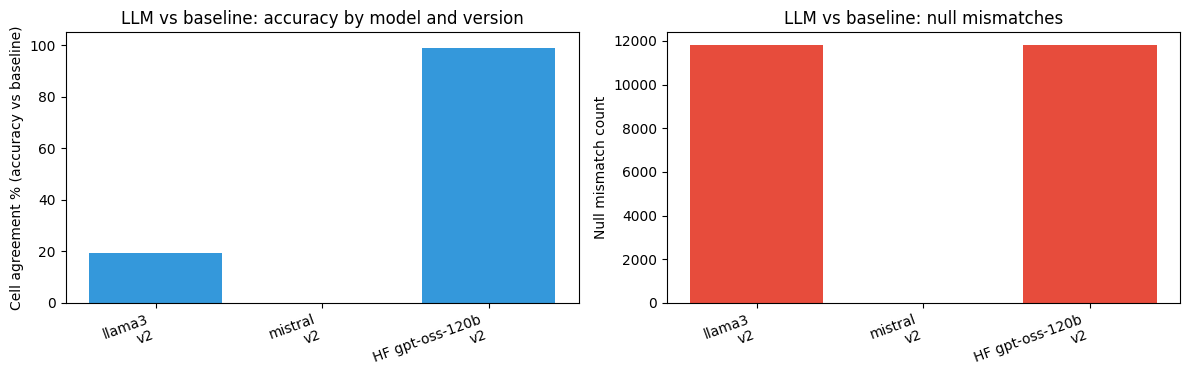
\includegraphics[width=0.9\textwidth]{figures/canonical_ingestion_llm_vs_baseline}
  \caption{Comparison of baseline vs.\ LLM-generated canonical ingestion for NYC taxi V2. Cell agreement (\%), row-count match, and per-column agreement are shown for \texttt{llama3}, \texttt{mistral}, and the Hugging Face \texttt{gpt-oss-120b} model. The baseline (deterministic mapping) serves as the reference; the HF model attains the highest cell-level agreement.}
  \label{fig:canonical-llm-vs-baseline}
\end{figure}

\begin{figure}[htbp]
  \centering
  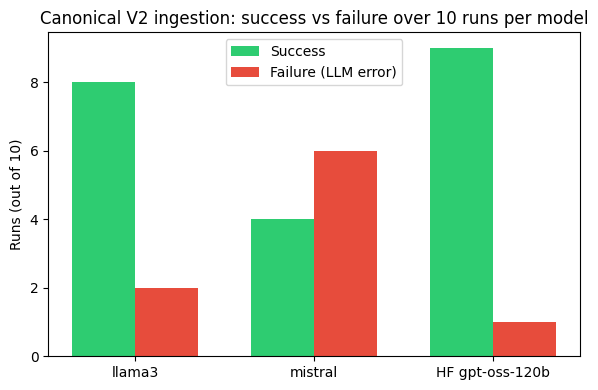
\includegraphics[width=0.9\textwidth]{figures/canonical_ingestion_success_runs.png}
  \caption{Ingestion success rate over multiple runs per model for the V2~$\rightarrow$~canonical scenario. Success indicates that the generated transform executed without error and produced a row count matching the baseline. The figure illustrates the variability of \texttt{llama3} and the more consistent success of the larger hosted model across runs.}
  \label{fig:canonical-ingestion-success-runs}
\end{figure}
\section{Ablation Results: Zero-Shot vs.\ RAG-Grounded Mapping}
\label{sec:results-ablation}

To isolate the effect of retrieval-augmented prompting from other design choices, an ablation study
was performed on the NYC taxi V2~$\rightarrow$~canonical ingestion scenario using the local
\path{llama3} model and the hosted Hugging Face model \path{openai/gpt-oss-120b:groq}. For each
model, five trials were run under a zero-shot condition (no retrieved schemas, change sets, or
reference code) and five trials under the full RAG-grounded condition described in
Section~\ref{sec:method-ablation}. Table~\ref{tbl:canonical-ablation-multi-model} summarises the
results in terms of average mapping accuracy, code executability, schema hallucinations, and
row-count match rate.

\begin{table}[h]
  \centering
  \caption{Ablation study: zero-shot vs. RAG-based canonical mappings for NYC taxi V2 across two LLM backends.}
  \label{tbl:canonical-ablation-multi-model}
  
  % This defines C as a centered wrapping column using standard LaTeX
  \newcolumntype{C}{>{\centering\arraybackslash}X}

  \begin{tabularx}{\textwidth}{>{\raggedright\arraybackslash}p{3cm} C C C C}
    \hline
    \textbf{Metric} & \textbf{llama3 (zero-shot)} & \textbf{llama3 (RAG)} & \textbf{gpt-oss-120B (zero-shot)} & \textbf{gpt-oss-120B (RAG)} \\
    \hline\hline
    Mapping accuracy (\%) & 0.0 & 19.8 & 58.1 & 98.8 \\
    Code executability (\%) & 0 & 20 & 100 & 100 \\
    Schema hallucinations (avg per run) & nan & 0.00 & 0.00 & 0.00 \\
    Runs with any schema hallucination (\%) & 0 & 0 & 0 & 0 \\
    Row-count match rate (\%) & 0 & 20 & 60 & 100 \\
    \hline
  \end{tabularx}
\end{table}

For \path{llama3}, the zero-shot condition failed in all runs: no generated transform compiled and
executed successfully, leading to an effective average accuracy of 0\% and a row-count match rate
of 0\%. Under the RAG-grounded condition, only one out of five runs executed successfully
(code executability 20\%), but that run achieved 98.85\% cell-level agreement with the deterministic
baseline, 100\% per-column agreement for all canonical attributes except \path{passenger_count},
and no schema hallucinations. The low average accuracy in Table~\ref{tbl:canonical-ablation-multi-model}
for \path{llama3} with RAG reflects this mixture of one near-perfect run and four failed runs.

In contrast, the \path{openai/gpt-oss-120b:groq} backend achieved 100\% code executability under
both prompting conditions. However, its zero-shot mappings were substantially less stable: average
accuracy was 58.1\% with a wide spread across runs, and only 60\% of runs produced the same row
count as the baseline. Several zero-shot runs mis-assigned timestamp and identifier fields or
produced inconsistent derived metrics, even though no extra (hallucinated) columns were introduced.
When grounded in schemas, change sets, and the reference transform snippet, the same model
consistently achieved 98.8\% cell-level agreement with the baseline, a 100\% row-count match rate,
and zero schema hallucinations across all runs.


\section{End-to-End AI-Assisted Workflow Results (RQ3)}
\label{sec:results-e2e}

The final set of results concerns the end-to-end AI-assisted workflow in which schema detection and mapping regeneration are integrated into an executable ETL pipeline. The JSONL file \path{results/e2e_ai_eval.jsonl} records, for each scenario and model, whether regeneration and pipeline execution succeeded, the total wall-clock duration of the AI-assisted path, and a small set of automatic quality checks on the resulting tables.

\subsection{Scenario: NYC Taxi V1~\texorpdfstring{$\rightarrow$}{->}~V2}

For the V1~$\rightarrow$~V2 scenario with canonical ingestion, three AI-assisted configurations are evaluated:
%
\begin{itemize}
  \item \textbf{\path{llama3}}: regeneration and pipeline execution both succeed with exit codes~0. The recorded duration is approximately 89.2~seconds, and the checks confirm a row count of 93{,}679 along with the presence of \path{trip_revenue} and \path{trip_duration_minutes}. The \path{non_negative_revenue} check passes, while the \path{non_negative_duration} check fails due to negative or zero durations in a small number of records, reflecting noisy source data rather than a logic error.
  \item \textbf{\path{mistral}}: regeneration and pipeline execution also succeed with exit codes~0. The recorded duration is approximately 142.4~seconds, again with a row count of 93{,}679 and the expected derived columns present. As with \path{llama3}, the \path{non_negative_duration} check fails due to outlier trips with implausible durations.
  \item \textbf{\path{openai/gpt-oss-120b:groq}} (Hugging Face router): regeneration and pipeline execution succeed with exit codes~0, resulting in the same row count and derived columns as the other models. The end-to-end duration is substantially lower, at around 6.4~seconds for regeneration plus pipeline execution in this controlled setting.
\end{itemize}

These results show that, for the evaluated taxi scenario, all three LLM configurations can be integrated into an end-to-end pipeline that completes successfully and produces tables passing basic automated checks, albeit with markedly different latency profiles.

Figure~\ref{fig:e2e-success-duration} summarises the end-to-end success rate and wall-clock duration for each model in the V1~$\rightarrow$~V2 scenario. All three configurations achieve a success rate of 1.0 under the database-level checks (row count, presence of \texttt{trip\_revenue} and \texttt{trip\_duration\_minutes}). The main difference lies in latency: the hosted \texttt{openai/gpt-oss-120b:groq} model completes regeneration and pipeline execution in approximately 6.4~seconds, whereas the local \texttt{llama3} and \texttt{mistral} models take on the order of 90--140~seconds. This figure supports the conclusion that the AI-assisted workflow is feasible across all evaluated backends, with hosted models offering a substantial speed advantage in this controlled setting.

\begin{figure}[htbp]
  \centering
  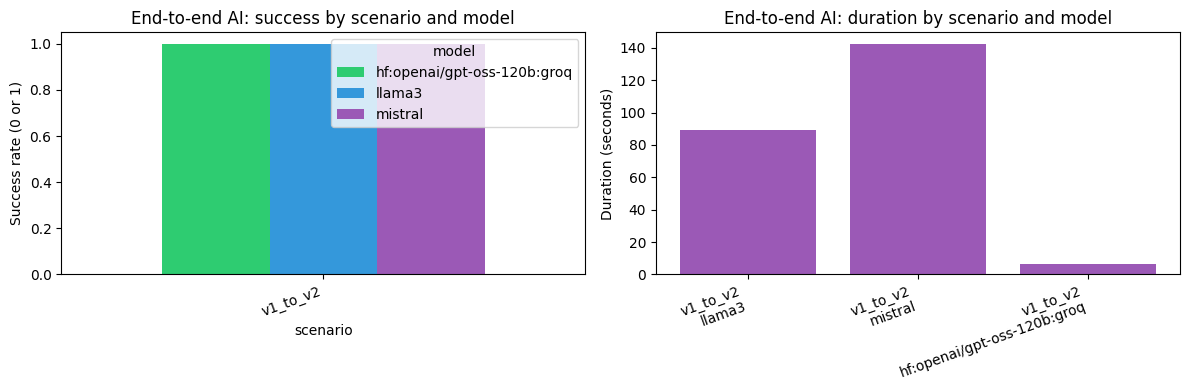
\includegraphics[width=0.85\textwidth]{figures/e2e_ai_success_duration}
  \caption{End-to-end AI-assisted workflow: success rate and duration per model for the NYC taxi V1~$\rightarrow$~V2 scenario. All models achieve full success under the automated DB checks; the bar chart highlights the large difference in wall-clock time between local (\texttt{llama3}, \texttt{mistral}) and hosted (\texttt{gpt-oss-120b}) backends.}
  \label{fig:e2e-success-duration}
\end{figure}

\section{Summary of Key Quantitative Metrics}
\label{sec:results-summary-table}

For ease of reference, Table~\ref{tbl:thesis-eval-summary} consolidates the most important quantitative metrics across schema detection (RQ1), canonical ingestion and mapping regeneration (RQ2), and the end-to-end AI-assisted workflow (RQ3). The values are derived from the evaluation scripts and the \path{thesis_evaluation_metrics.ipynb} notebook.

\begin{table}[h]
  \centering
  \caption{Summary of thesis-wide evaluation metrics across schema detection, canonical ingestion, and end-to-end AI-assisted execution.}
  \label{tbl:thesis-eval-summary}
  % \tabularx{total width}{column types}
  % 'X' columns will expand/contract to fill the remaining space and wrap text.
  \begin{tabularx}{\textwidth}{@{} l X l r l @{}}
    \toprule
    \textbf{Part} & \textbf{Scenario / Version} & \textbf{Metric} & \textbf{Value} & \textbf{Reference} \\
    \midrule
    1. Schema detection & \path{canonical\_v2} & F$_{1}$ (overall) & 1.00 & Ground truth \\
    2. Baseline vs. LLM & \path{llama3 / v2} & Cell agreement \% & 19.50 & Baseline alg. \\
    2. Baseline vs. LLM & \path{mistral / v2} & Cell agreement \% & 0.00 & Baseline alg. \\
    2. Baseline vs. LLM & \path{HF gpt-oss-120b / v2} & Cell agreement \% & 98.85 & Baseline alg. \\
    \addlinespace
    3. E2E AI & \path{v1\_to\_v2 / llama3} & Success & 1.00 & DB checks \\
    3. E2E AI & \path{v1\_to\_v2 / llama3} & Duration (s) & 89.17 & Wall clock \\
    3. E2E AI & \path{v1\_to\_v2 / mistral} & Success & 1.00 & DB checks \\
    3. E2E AI & \path{v1\_to\_v2 / mistral} & Duration (s) & 142.43 & Wall clock \\
    3. E2E AI & \path{v1\_to\_v2 / gpt-oss-120b:groq} & Success & 1.00 & DB checks \\
    3. E2E AI & \path{v1\_to\_v2 / gpt-oss-120b:groq} & Duration (s) & 6.40 & Wall clock \\
    \bottomrule
  \end{tabularx}
\end{table}


